\documentclass[a4paper,20pt,titlepage]{article}
\usepackage[utf8]{inputenc}
\usepackage{float}
\usepackage{amsmath}
\usepackage{graphicx}
\usepackage[margin=0.8in]{geometry}
\usepackage[breaklinks]{hyperref}
\usepackage{listings}
\usepackage{pdfpages}
\usepackage{comment}
\usepackage{fancyhdr}
\usepackage[english]{babel}
\usepackage{subcaption}
\begin{document}

\begin{titlepage}
   \begin{center}
   
        \huge
       \textbf{Habib University} \\
       \textbf{Dhanani School of Science and Engineering} \\
       
        \begin{figure}[H]
           \centering
           
\includegraphics[scale = 0.75]{HU logo.jpg}
           \label{fig:my_label}
       \end{figure}

        \vspace{0.5cm}

         \textbf{CS 201 - Data Structures II}
         \vspace{0.5cm}

         \LARGE
         \textbf{Course Instructor:}
         
         \Large
         Muhammad Mobeen Movania	

        \vspace{1cm}
        \huge
        \textbf{Phylogenetics using an Inverted Index}
        
      \vspace{1cm}
      \Large
      by       
      \vspace{1cm}
      
      \Large{Ifrah Chishti\footnote{Student ID: 08351, Email: ic08351@st.habib.edu.pk}, Kulsoom Asim\footnote{Student ID: 08051, Email: ka08051@st.habib.edu.pk}, M. Moaz Siddiqui\footnote{Student ID: 08084, Email: ms08084@st.habib.edu.pk}, Rohaan Khan\footnote{Student ID: 08102, Email: ra08102@st.habib.edu.pk}}
      \vspace{1cm}
      
      \today \\
      
   \end{center}
\end{titlepage}
\cfoot{\thepage}
\tableofcontents
\newpage

\section{Introduction}

In the realm of biological research, efficient management of primate data, characterized by diverse attributes like species name, habitat, diet, and behavior, is crutial for understanding their ecology and behavior. Using an inverted index as a data structure offers a solution to this challenge. By indexing each attribute along with corresponding data entries, the inverted index enables rapid retrieval and manipulation of primate data based on specific criteria.

This indexing mechanism supports complex querying and filtering operations, allowing researchers to extract relevant subsets of data efficiently. Furthermore, the scalability of inverted index structures accommodates the continuous influx of new data, ensuring that research efforts remain dynamic and up-to-date. In summary, the utilization of inverted index data structures enhances the efficiency of primate data management, accelerates research workflows, and contributes to a deeper understanding of primate ecology and evolution.


\section{What is an Inverted Index?}
An inverted index is a database index that maps content, such as words or numbers, to their locations in a document, table, or set of documents. This data structure is used to store and organize information for efficient search and retrieval. Inverted indexes are an important part of search engines and information retrieval systems, and are used to facilitate more efficient full-text searches in a database.

\section{Phylogenetic Tree}
The graph of primate evolution, often depicted as a phylogenetic tree, serves as a visual roadmap tracing the evolutionary relationships among primate species. This tree, constructed based on genetic, morphological, and fossil evidence, illustrates the branching patterns and divergence points in primate evolution. Each branch represents a distinct lineage, while nodes indicate common ancestors shared by multiple species. Through the phylogenetic tree, scientists can infer the evolutionary history of primates, deciphering the sequence of speciation events and understanding the evolutionary processes driving primate diversification. This tree not only elucidates the origins and relationships of modern primate taxa but also provides insights into the broader context of mammalian evolution and the interconnectedness of life on Earth \cite{KhanAcademy}.

\section{Constructing the tree}
We first collected data on characteristics \cite{NHC} that helped in distinguishing each superfamily.
In doing so we group the species into less and less inclusive clads \cite{Berkeley}.
We included the following characteristics for the following tree:

\begin{itemize}
  \item Flattened nails
  \item Reduced olfactory mechanism
  \item Collarbone
  \item Bipedalism
  \item Sit upright
  \item Upright Standing Gait
  \item Specialized tooth-comb
  \item Down-Ward Facing Nostril
  \item Extremely Large Eyes
\end{itemize}

\begin{figure}[htbp]
    \centering
    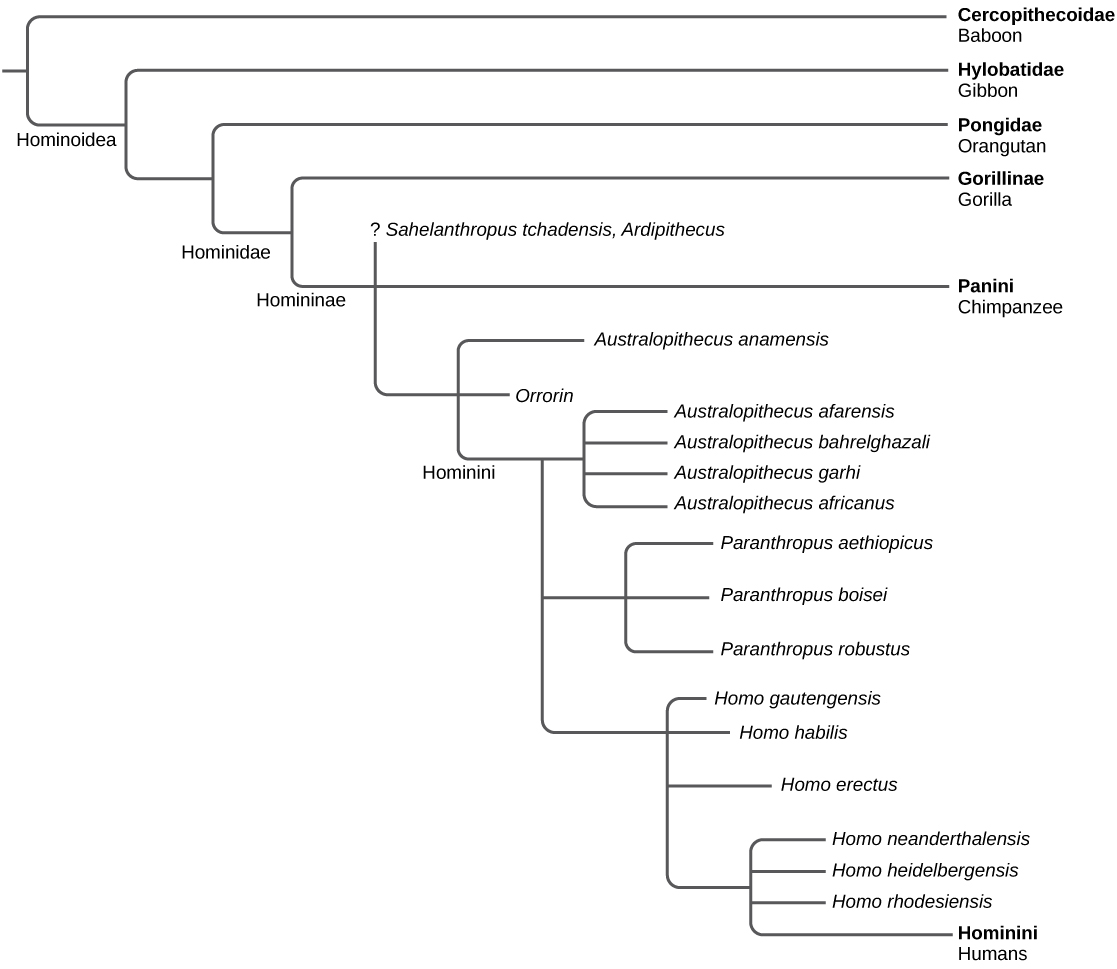
\includegraphics[width=0.5\textwidth]{primates.jpg}
    \caption{Phylogenetic tree}
    \label{fig:example}
\end{figure}


\section{GUI Interface for Comparison}

We designed a comparison index by which the similarity of 2 species can be checked, with and index of 1 meaning that the 2 species are very similar and 0 meaning that the species have very little in common, and thus, are not closely related.

\begin{figure}[htbp]
    \centering
    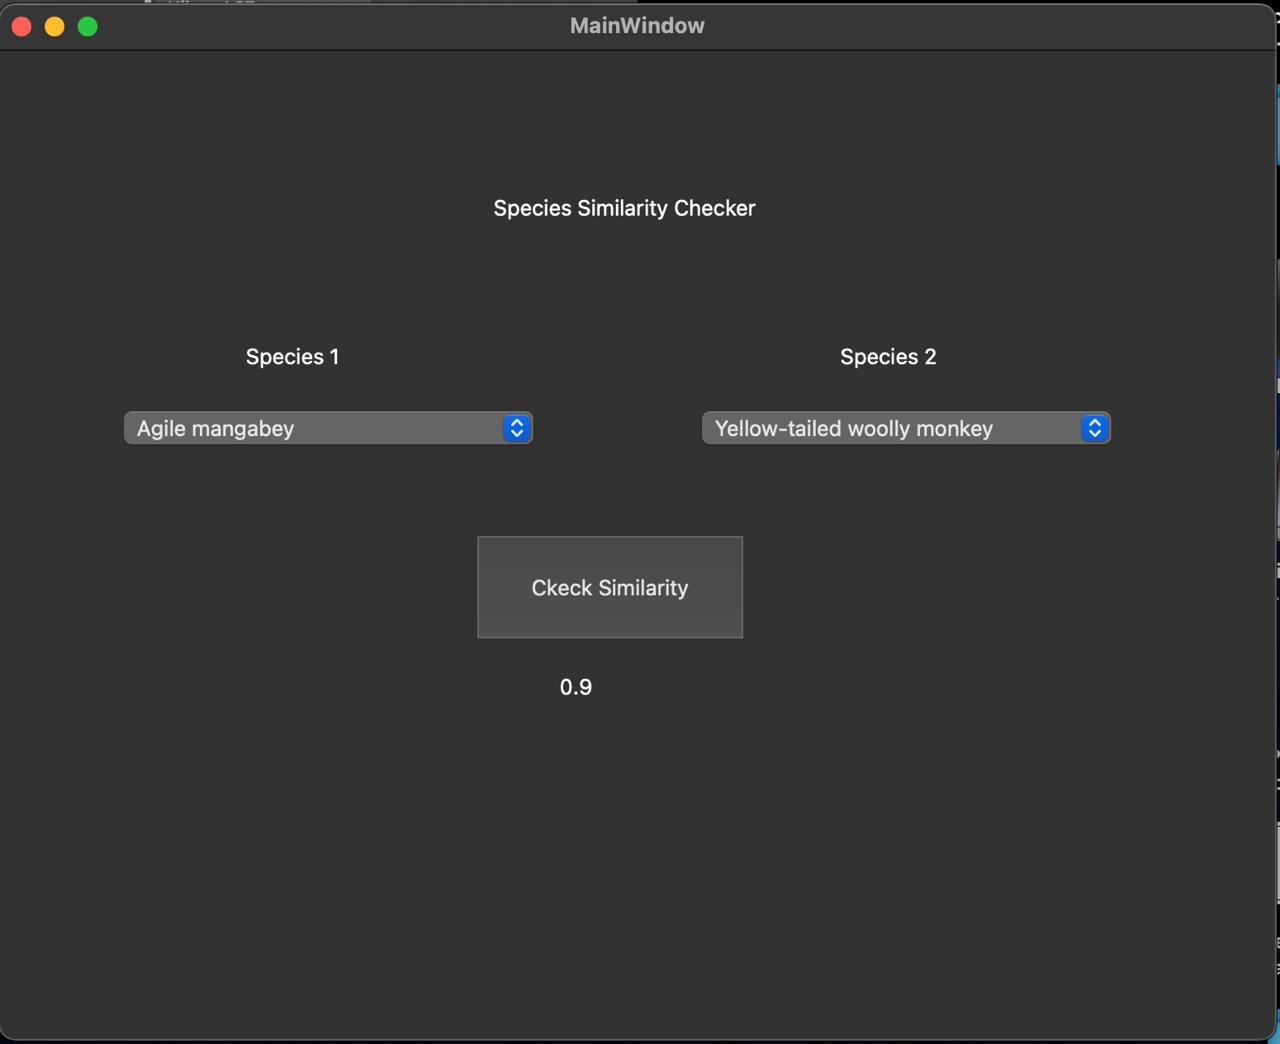
\includegraphics[width=0.5\textwidth]{1.jpg}
    \caption{GUI Implementation}
    \label{fig:example}
\end{figure}

\section{Conclusion}
The project showcases the effectiveness of inverted index data structure in managing primate data based on their attributes. With the implemented functionalities and potential future enhancements, the system provides a powerful tool for primate researchers, conservationists, and enthusiasts to explore, analyze, and contribute to the understanding and conservation efforts of primate species worldwide.


\section{GitHub}
The code for our project can be found in the following GitHub repository:

\noindent
\url{https://github.com/MuhammadMoazSiddiqui08084/DS2-Project}


\bibliographystyle{plain}
\bibliography{refs}
\end{document}